\newpage
\section{Threshold and edge detection}
To measure a object bypassing the camera field the outlines of the object are needed. The challenge here is to find the edges of an object with little computing power in such a short time that the measurement time does not become useless. For further processing the edges have to be represented by an one pixel thick line. This section shows the used method and implementation of the further used edge detection. The ISP driver of the Jetson Nano is used in the automatic mode. In this configuration the ISP tries to keep the mean of the image close to the value 128, which resembles the middle of its range. Since the gStreamer pipeline handling over Python is somewhat complicated, the camera is only used in automatic mode.

\subsection{Threshold}
To determine a good threshold method a short look at the histogram is the first step to success. With a back light it can be expected to have a clear difference between foreground and background of the image. 
\begin{figure}[H]
	\subfigure[\label{development:thre1}]{\fbox{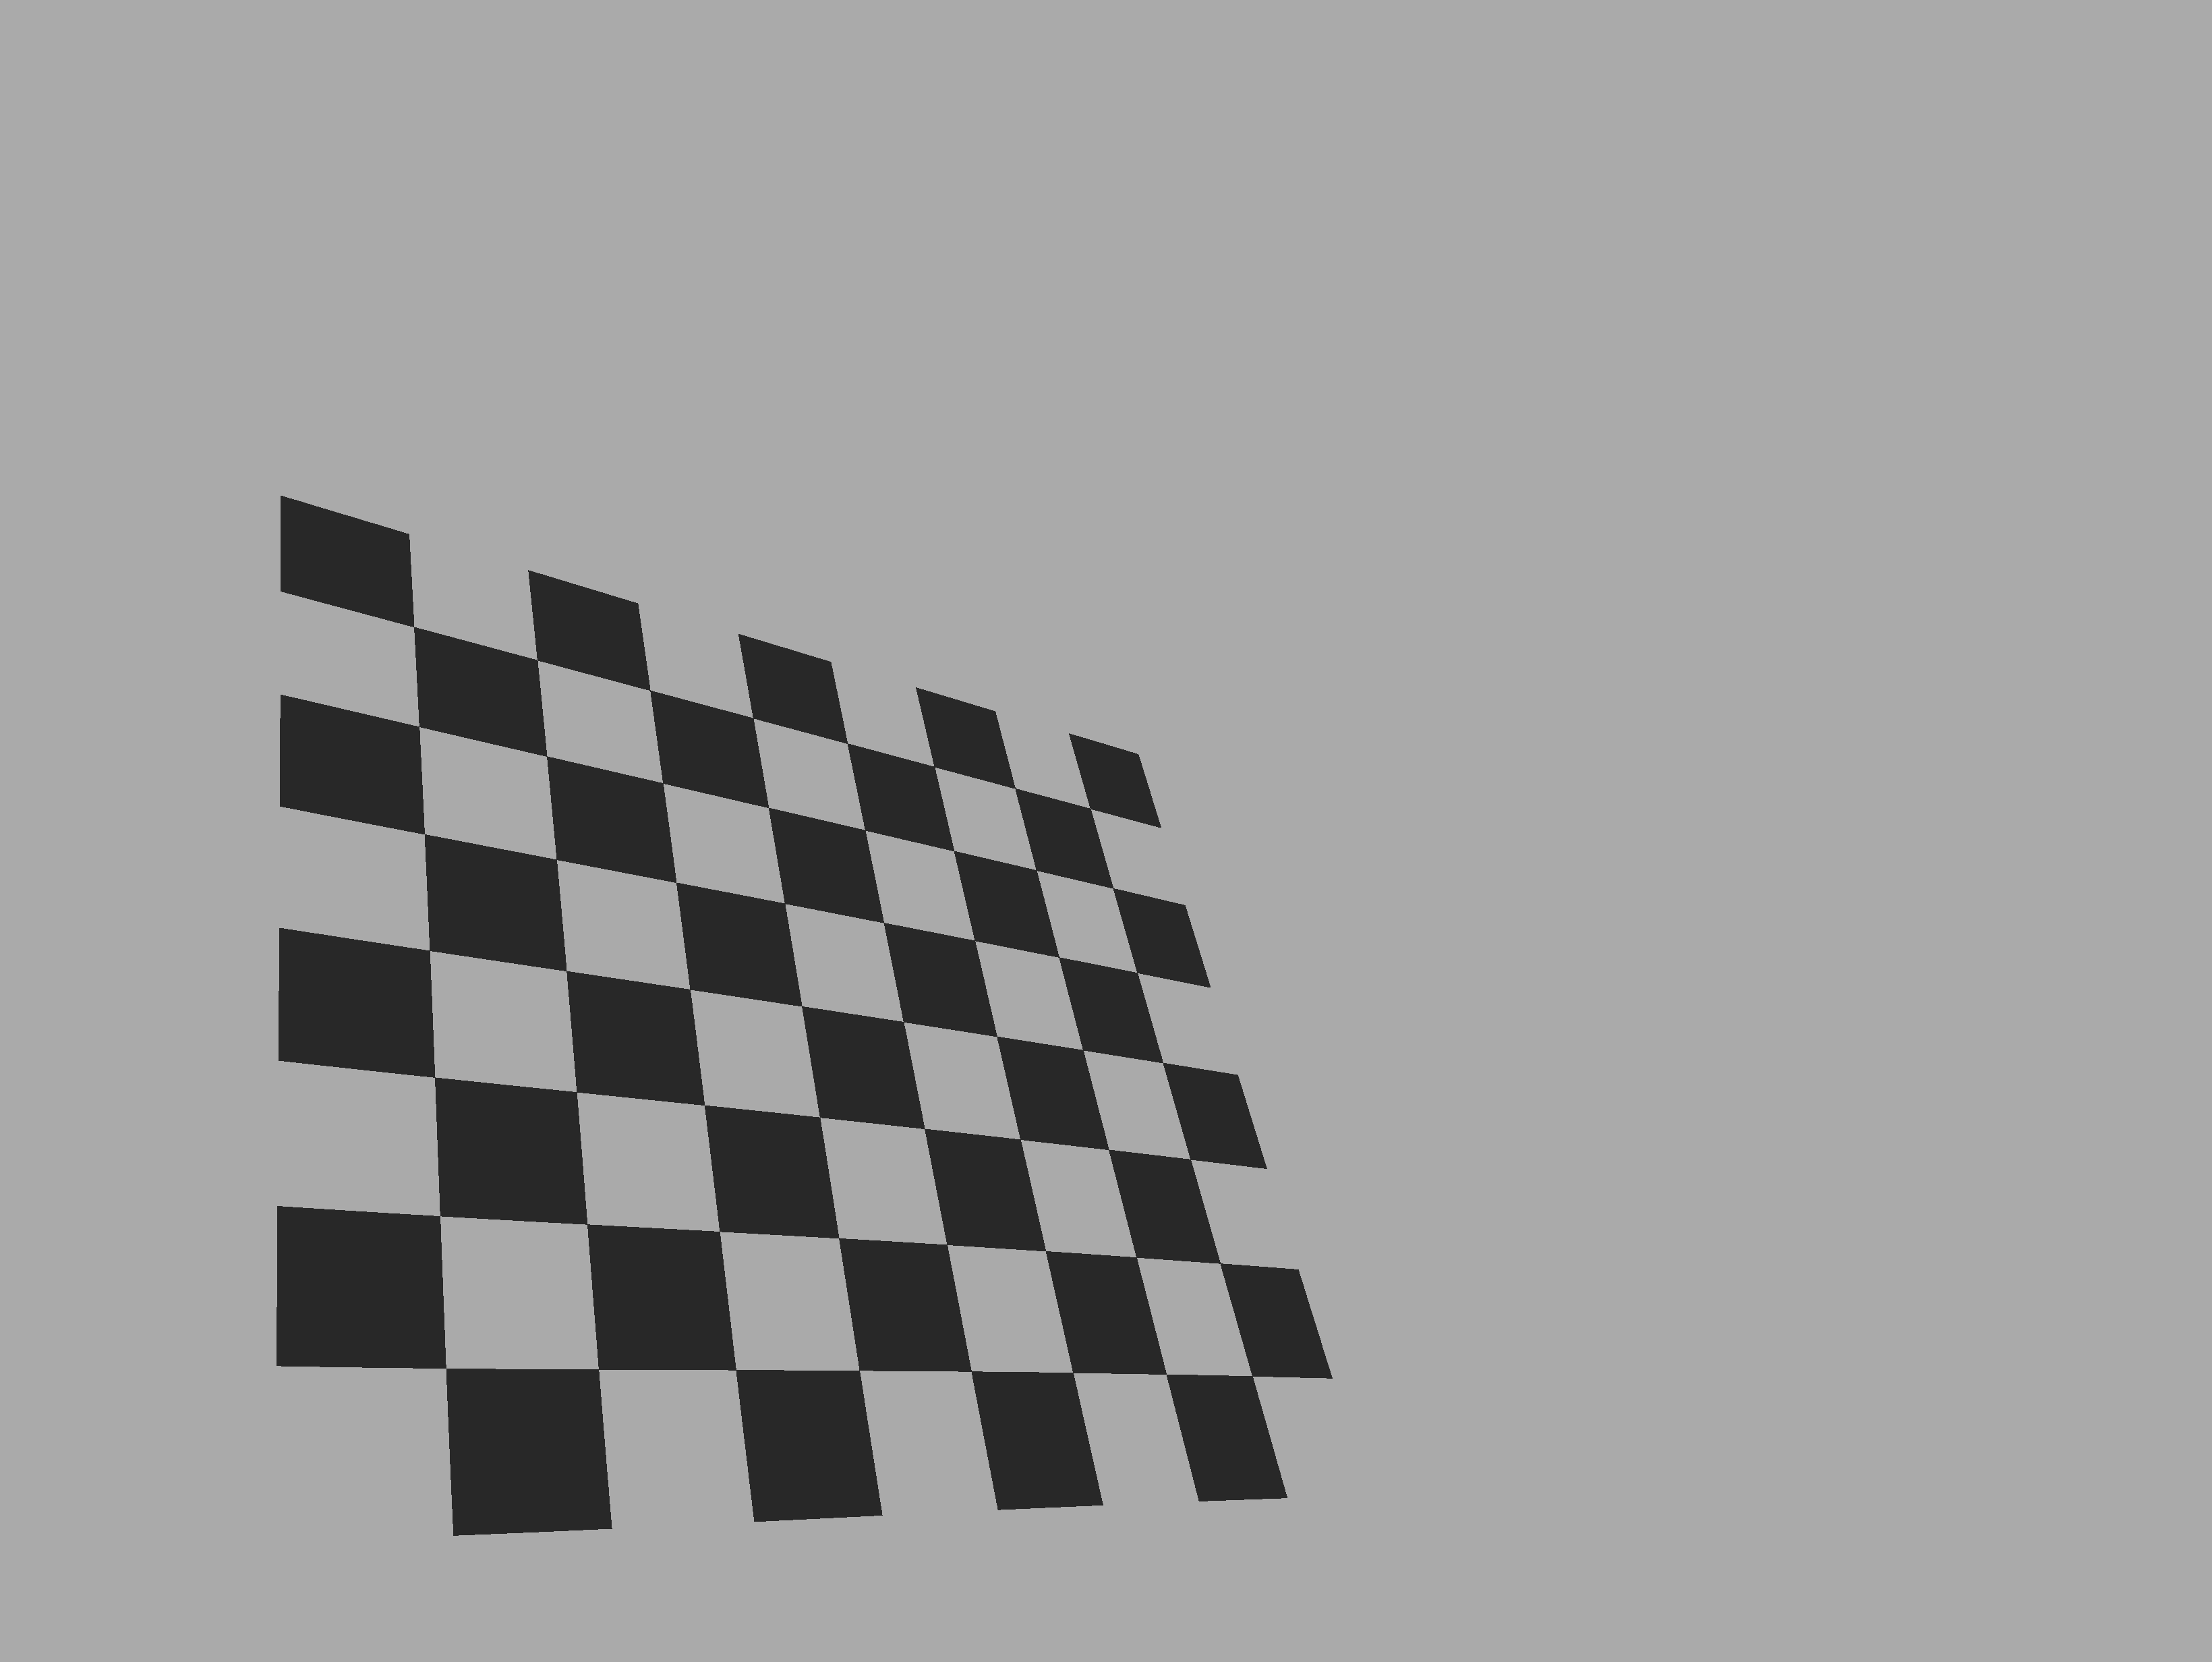
\includegraphics[width=0.5\linewidth, height=5cm]{3-development/threshold/im0.png}}}
	\subfigure[\label{development:thre2}]{\fbox{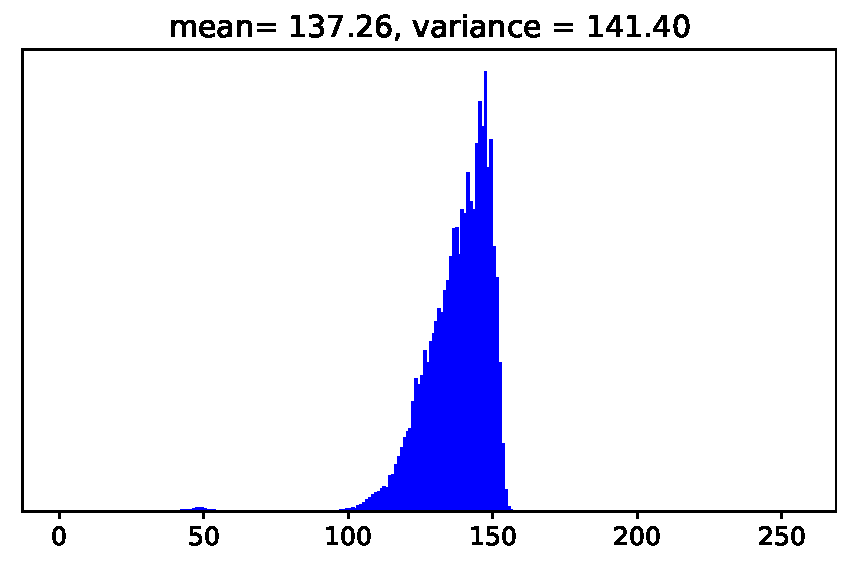
\includegraphics[width=0.5\linewidth, height=5cm]{3-development/threshold/hist_pattern2.pdf}}}
	\subfigure[\label{development:thre3}]{\fbox{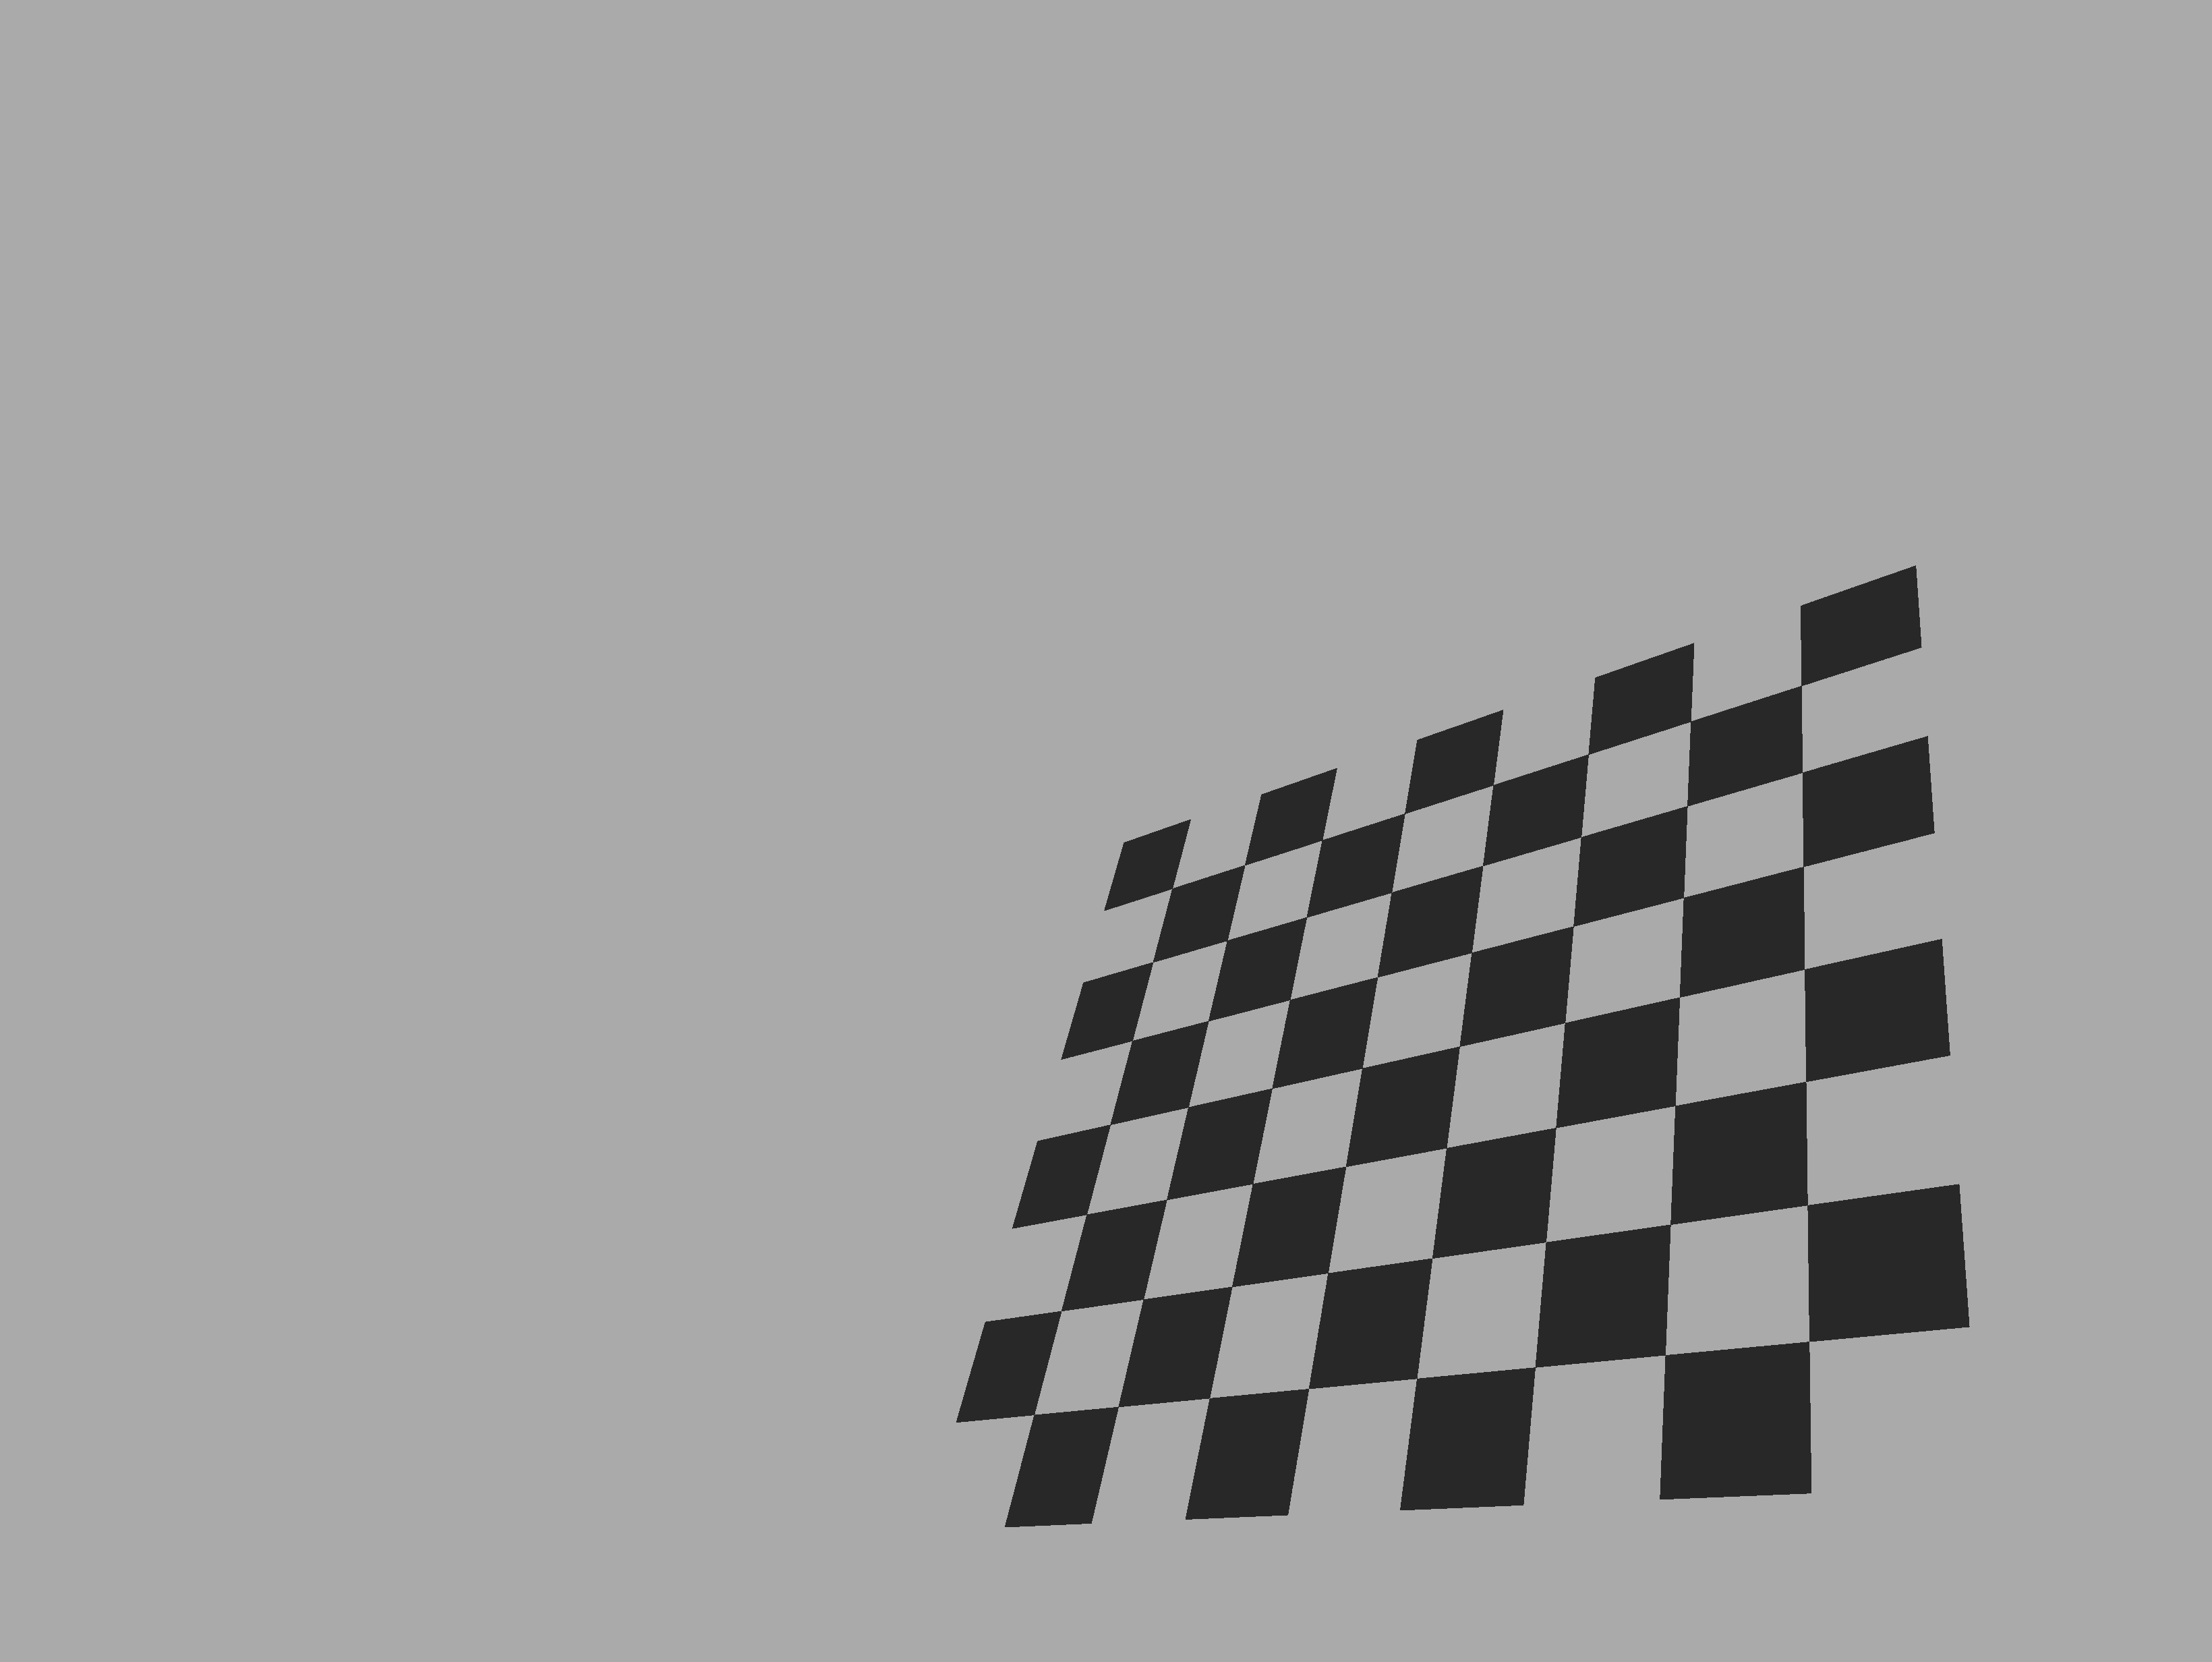
\includegraphics[width=0.5\linewidth, height=5cm]{3-development/threshold/im1.png}}}
	\subfigure[\label{development:thre4}]{\fbox{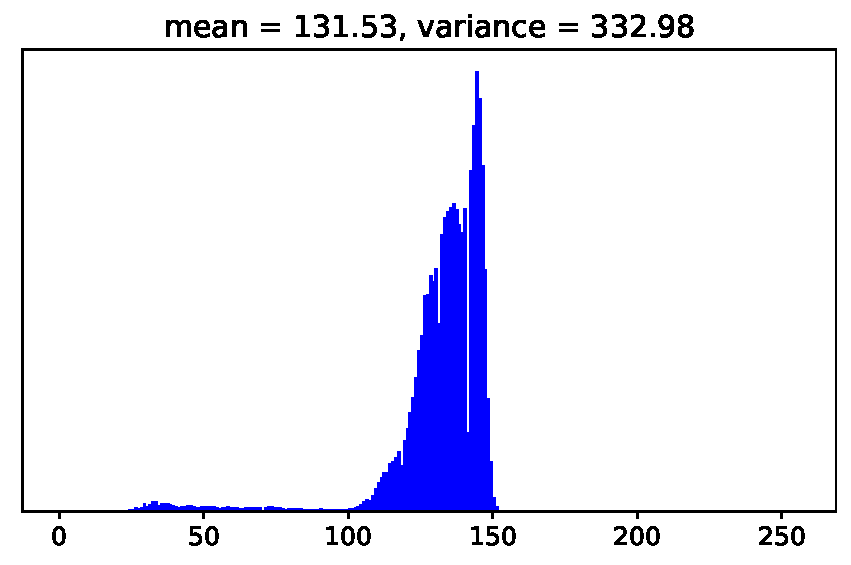
\includegraphics[width=0.5\linewidth, height=5cm]{3-development/threshold/hist_feder2.pdf}}}
	\caption{Histogram of the reference pattern and a spring with running back light\label{development:thre}}	
\end{figure}
\newpage
In the picture \ref{development:thre1} the back light is running and the calibration pattern is in place but no object to measure. The corresponding histogram \ref{development:thre2} shows that nearly every pixel belongs to the background white which is between the value 100 and 155. If a object enters the field of view of the camera it is displayed as black and we get more small values. This shift is also reproduced by the variance. The mean itself is getting corrected by the ISP and can not be used to detect if an object is in the image or not.\\
The obvious answer for a threshold would now be to just cut the histogram around the value 100 in two and set the values to black and white. But with the automatic ISP there is a good chance to loose important information if there is no adaptive threshold. Since the goal is to get as much information as possible from the edges, a little bit of noise can be handled. The method which produced the best results with a back light, was the triangle method \ref{theory:triangle}.

The triangle method calculates the value 112 on the given image \ref{development:thre3} which, using a binary threshold, results in the image \ref{development:thresh}. It is visible that we get a lot of noise in the edges of the resulting picture. \\
\begin{center}
	%\centering
	\fbox{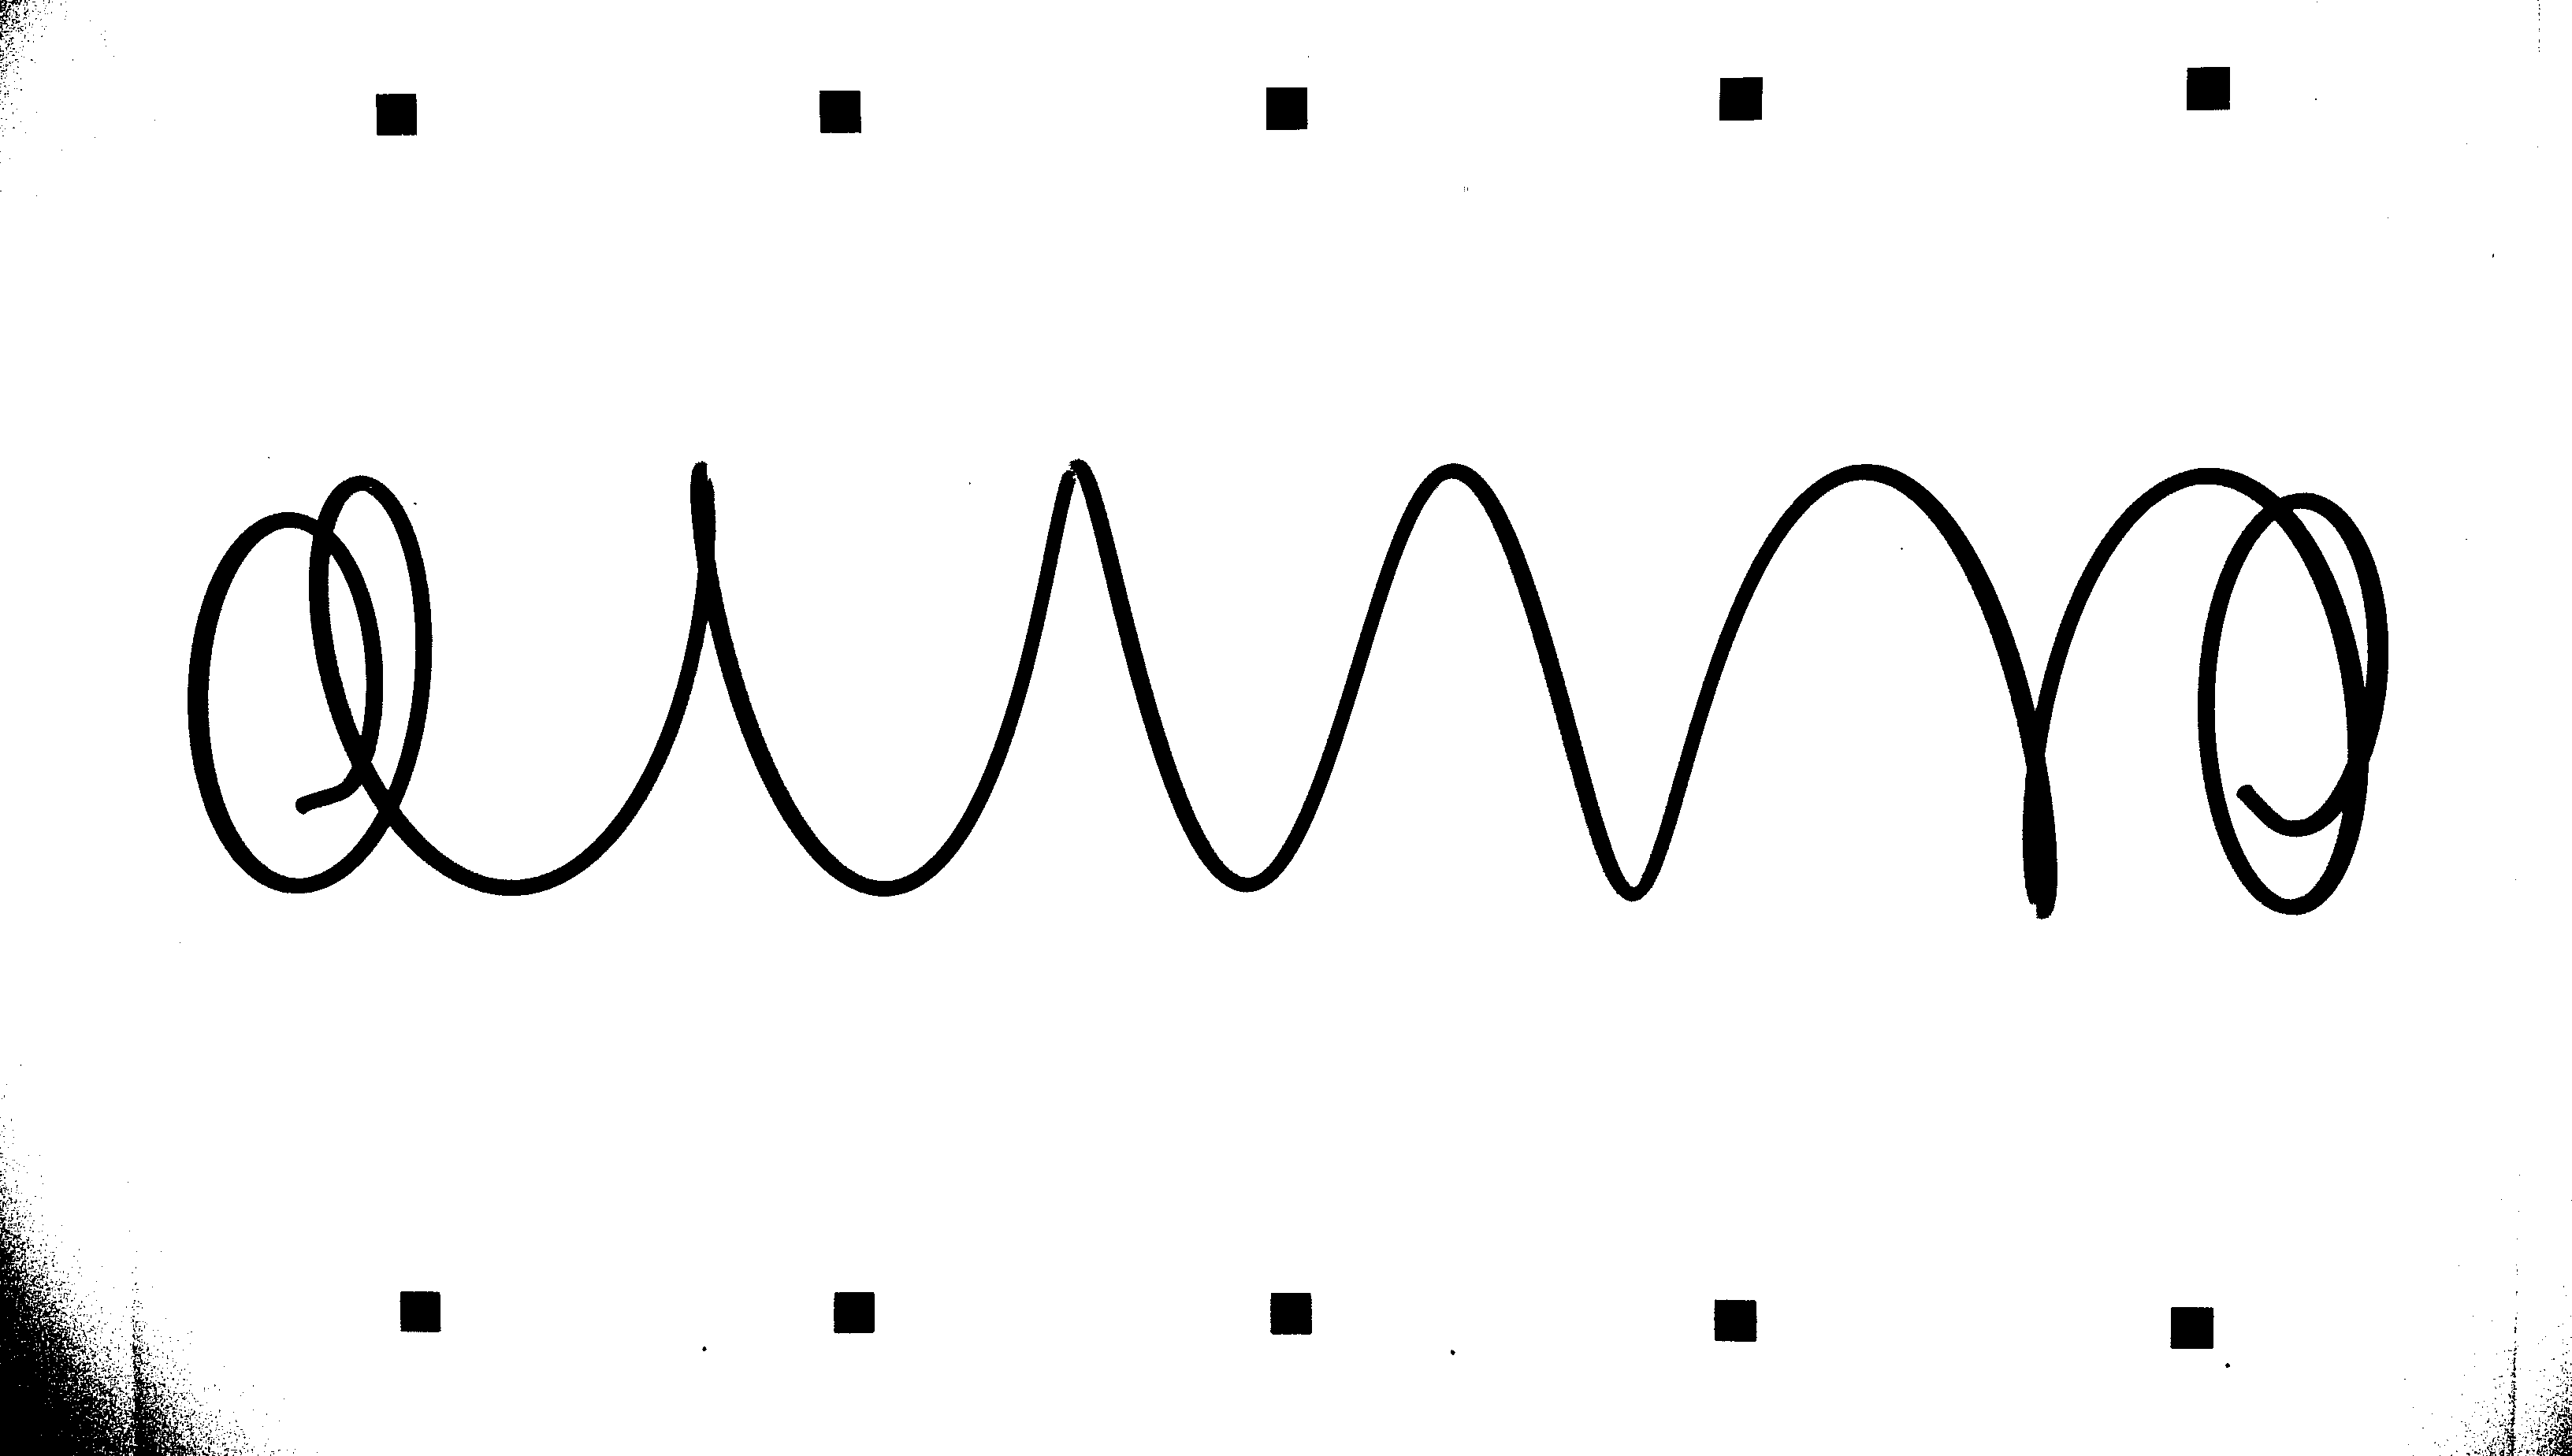
\includegraphics[width=0.9\linewidth]{3-development/threshold/threshold.png}}
	\captionof{figure}{Image after triangle threshold with threshold value 112}
	\label{development:thresh}
\end{center}
since the noise occurs only in the edges of the image it can dealt with ease. The focus lies more on the pattern and spring which should lose as few information as possible.

Another very popular method for an global adaptive threshold is the otsu algorithm. Otsu's goal is to maximize the variance of the fore and background in a image as good as possible in the histogram. Also known as the between-class variance. The result of an otsu threshold on the given image \ref{development:thre3} can be seen in the image \ref{development:otsu}. On the first sight it looks pretty clean and no noise is visible. Which leads to think that the otsu should be a good algorithm for this problem. But if the images \ref{development:triangle} and \ref{development:otsu} are investigated a little bit closer and compared directly it shows some disadvantage of the otsu which can not be corrected afterwards.\\


\begin{figure}[!h]
	\subfigure[\label{development:triangle}]{\fbox{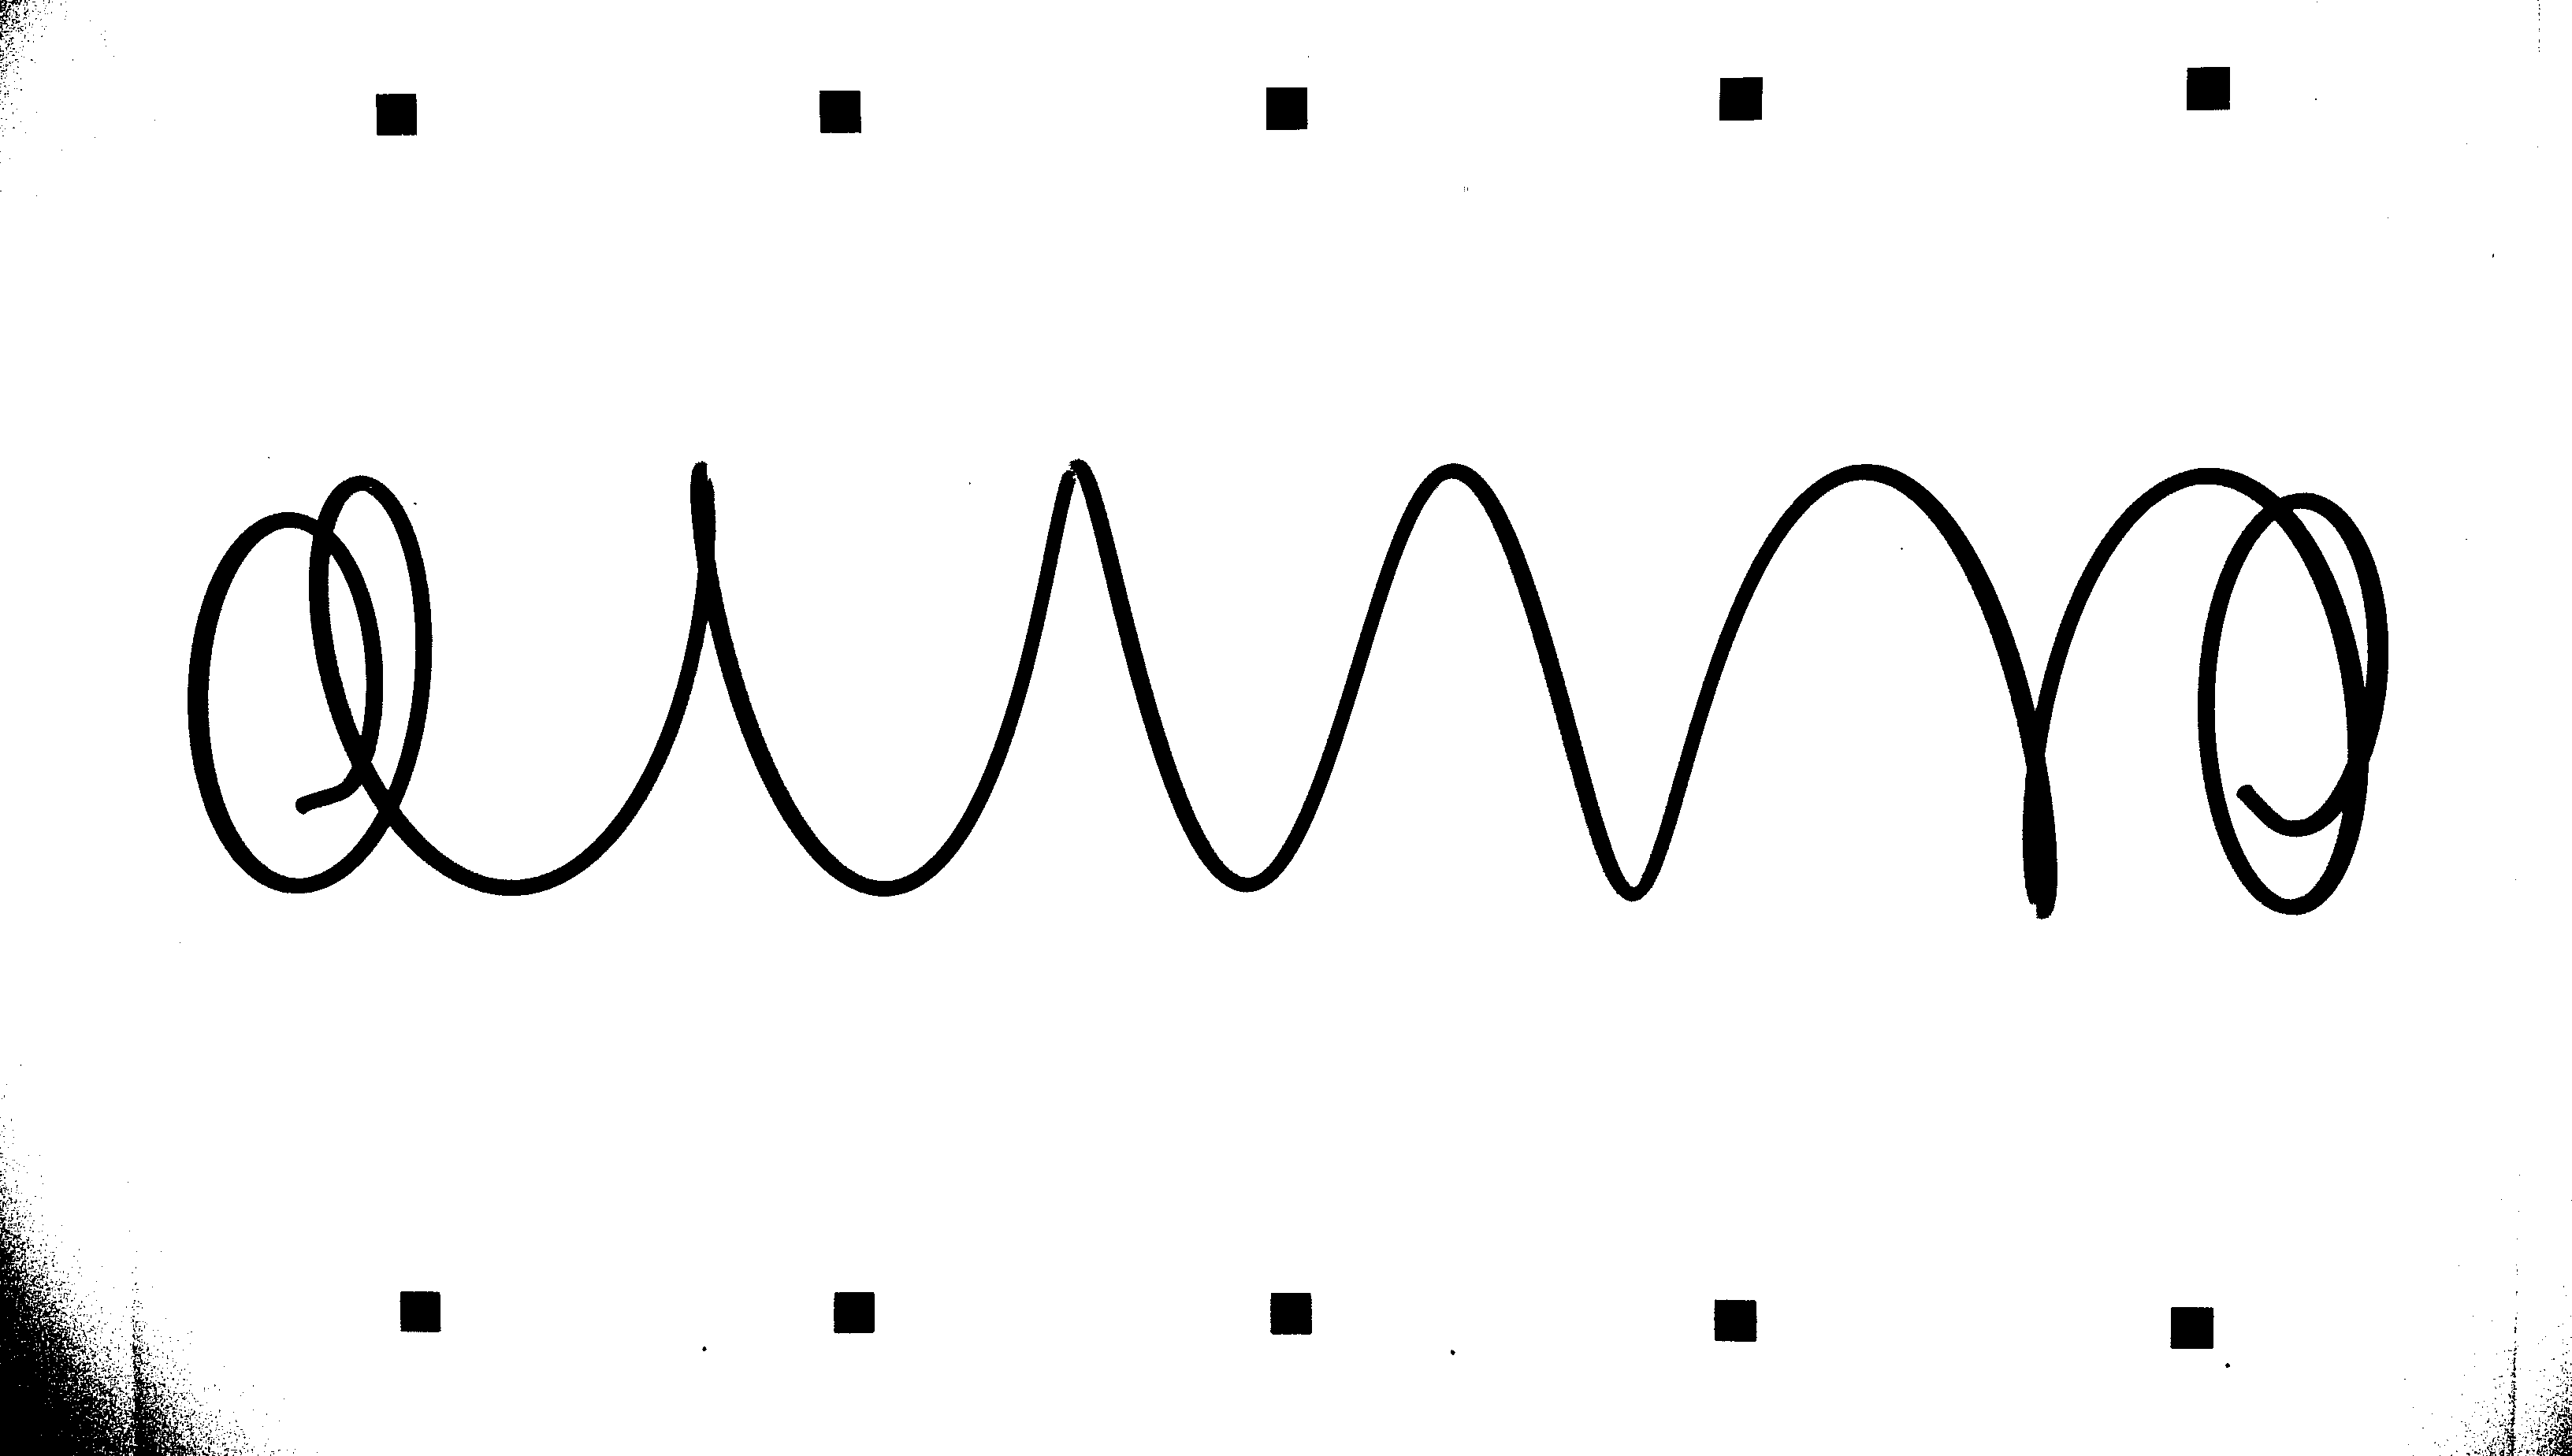
\includegraphics[width=0.45\linewidth, height=5cm]{3-development/threshold/threshold.png}}}
	\subfigure[\label{development:otsu}]{\fbox{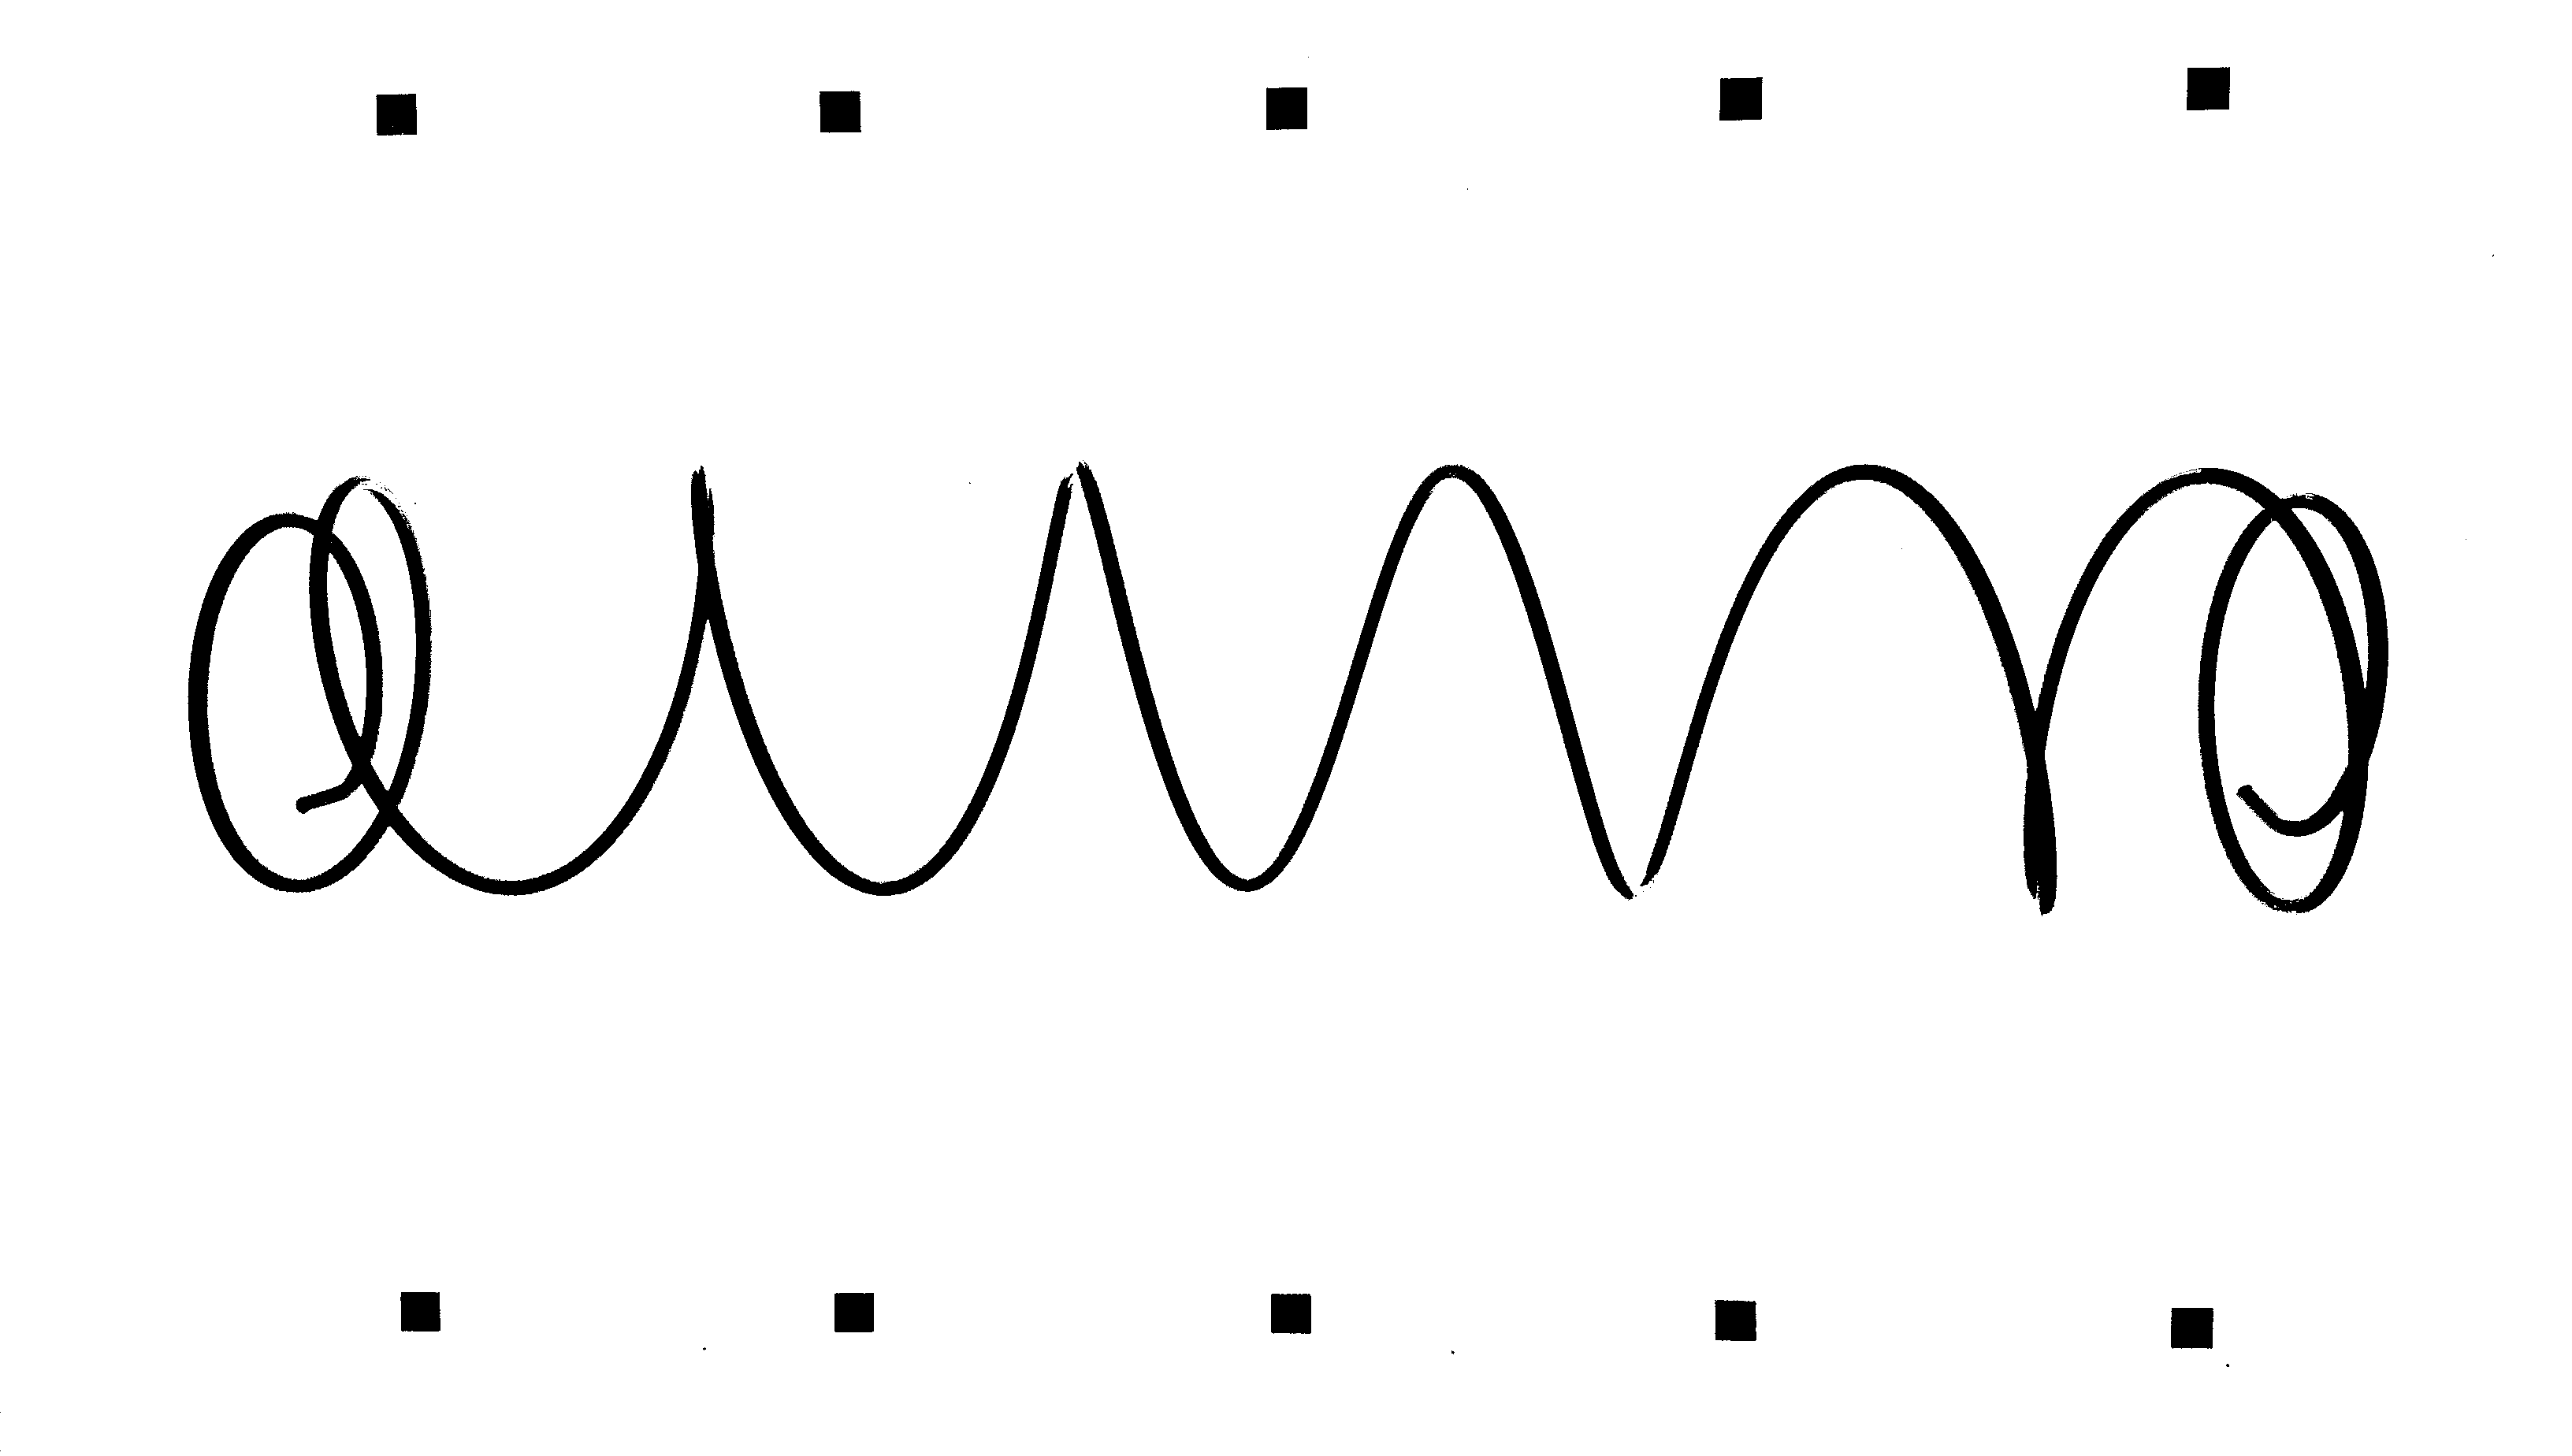
\includegraphics[width=0.45\linewidth, height=5cm]{3-development/threshold/otsu.png}}}
	\subfigure[\label{development:difference}]{\fbox{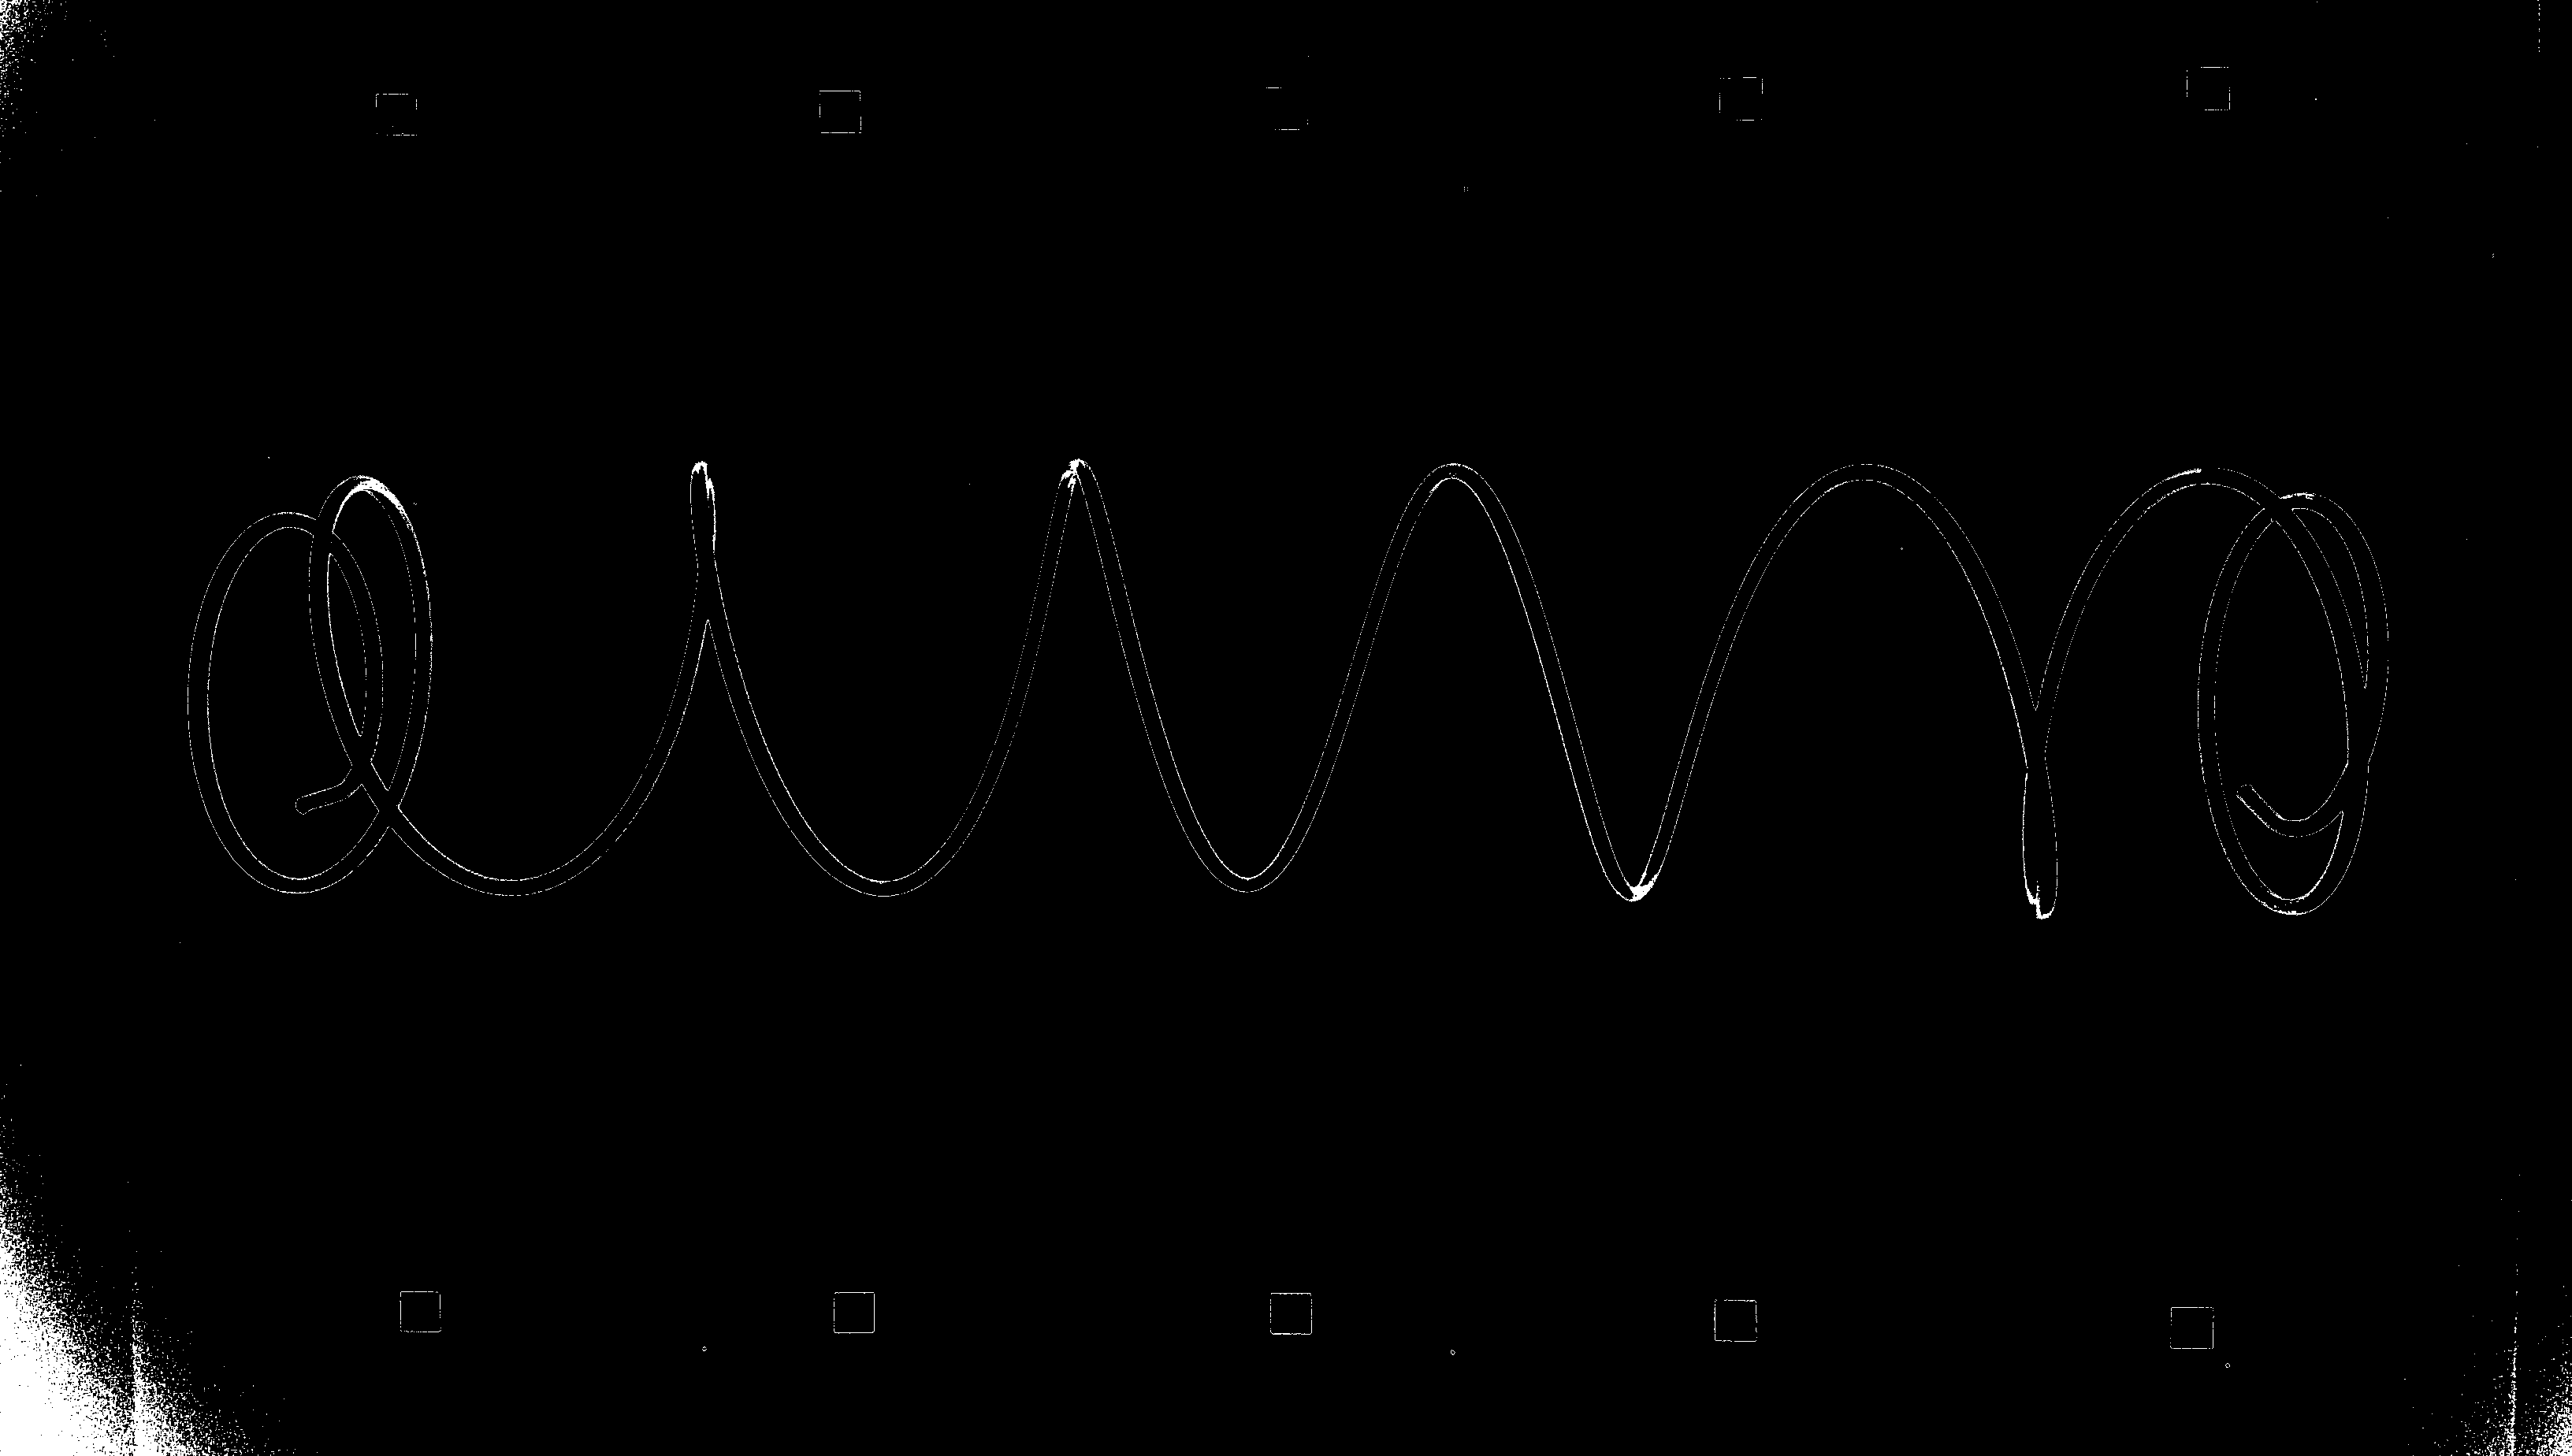
\includegraphics[width=1\linewidth]{3-development/threshold/diff.png}}}
	\caption{Comparison between otsu and triangle threshold\label{development:diff}}	
\end{figure}

If we look closely at the silhouette of the spring after the otsu threshold it seems that in some parts of the spring are disappearing. While the spring in thresholded with the triangle method seems far less effected from this effect. To better illustrate this effect the otsu image is subtracted by the triangle one which results in the difference image \ref{development:difference}.  
Now the difference clearly shows how much information is lost on the edges of the spring and even on the pattern. This information once lost can not be obtained again. With this in mind the otsu seems unsuitable for this problem. \\
The source of the problem itself is that the spring reflects the stray light of the backlight. The stray light is produced by two effects, one is the diffusion film which is only 4mm away from the spring. The second one is the reflected light from the construction itself. Meaning the top of the construction where the camera is mounted reflects some amount back on the spring. These two sources of stray light are leading to the spring being illuminated enough from the top, that some brightness values captured by the camera sensor are the same in the edges of the image as parts of spring.\\
Hardware improvements to minimize this problem would be to use light control filters which results in higher hardware cost. Another way would be to increase the distance between the glass the spring slides over and the diffusion filter so less stray light appears. In additional to these two solution the backlight could be changed so to more LED's in the corner of the PCB. Resulting in a backlight which is brighter in the corners as in the center. While the camera gets less light in the corner called vignetting. This backlight would reduce the vignetting of the camera to a certain amount. \\
Vignetting can also be handled in software. Since the background of the image stays the same it is possible to subtract the background of the image first eliminating the noise in the corner. The down side in correcting the brightness in a complex manner is the time spent doing it. Since every pixel have to be corrected it takes a good amount of time for the whole image. This would reduce the speed of the whole measurement drastically. \\

\subsection{Edge detection}   
To obtain the edge from a thresholded image morphological algorithms are very fast. Thanks to the good threshold results which also uses quite some time to calculate it is now fairly easy to get the edge of the spring. To extract the boundary of the spring we use a 3x3 kernel to erode the given image. The kernel $K$ is shaped as followed:
\begin{center}
\setlength{\tabcolsep}{0.5em} % for the horizontal padding
{\renewcommand{\arraystretch}{1.2}
\begin{tabular}{|c|c|c|}
	\hline
	1&1&1\\
	\hline
	1&1&1\\
	\hline
	1&1&1\\
	\hline
\end{tabular}
}
\end{center}

This kernel $K$ is used to erode the image and subtract the eroded image from the starting image. Lets name the thresholded image $T$. The math done is 
\begin{align*}
 E = T-(T\ominus K)
\end{align*}
returning the image containing all the edges $E$. In our example picture the resulting picture $E$ is displayed in the image \ref{development:edge}.\\



\begin{figure}[!h]
	\centering
	\fbox{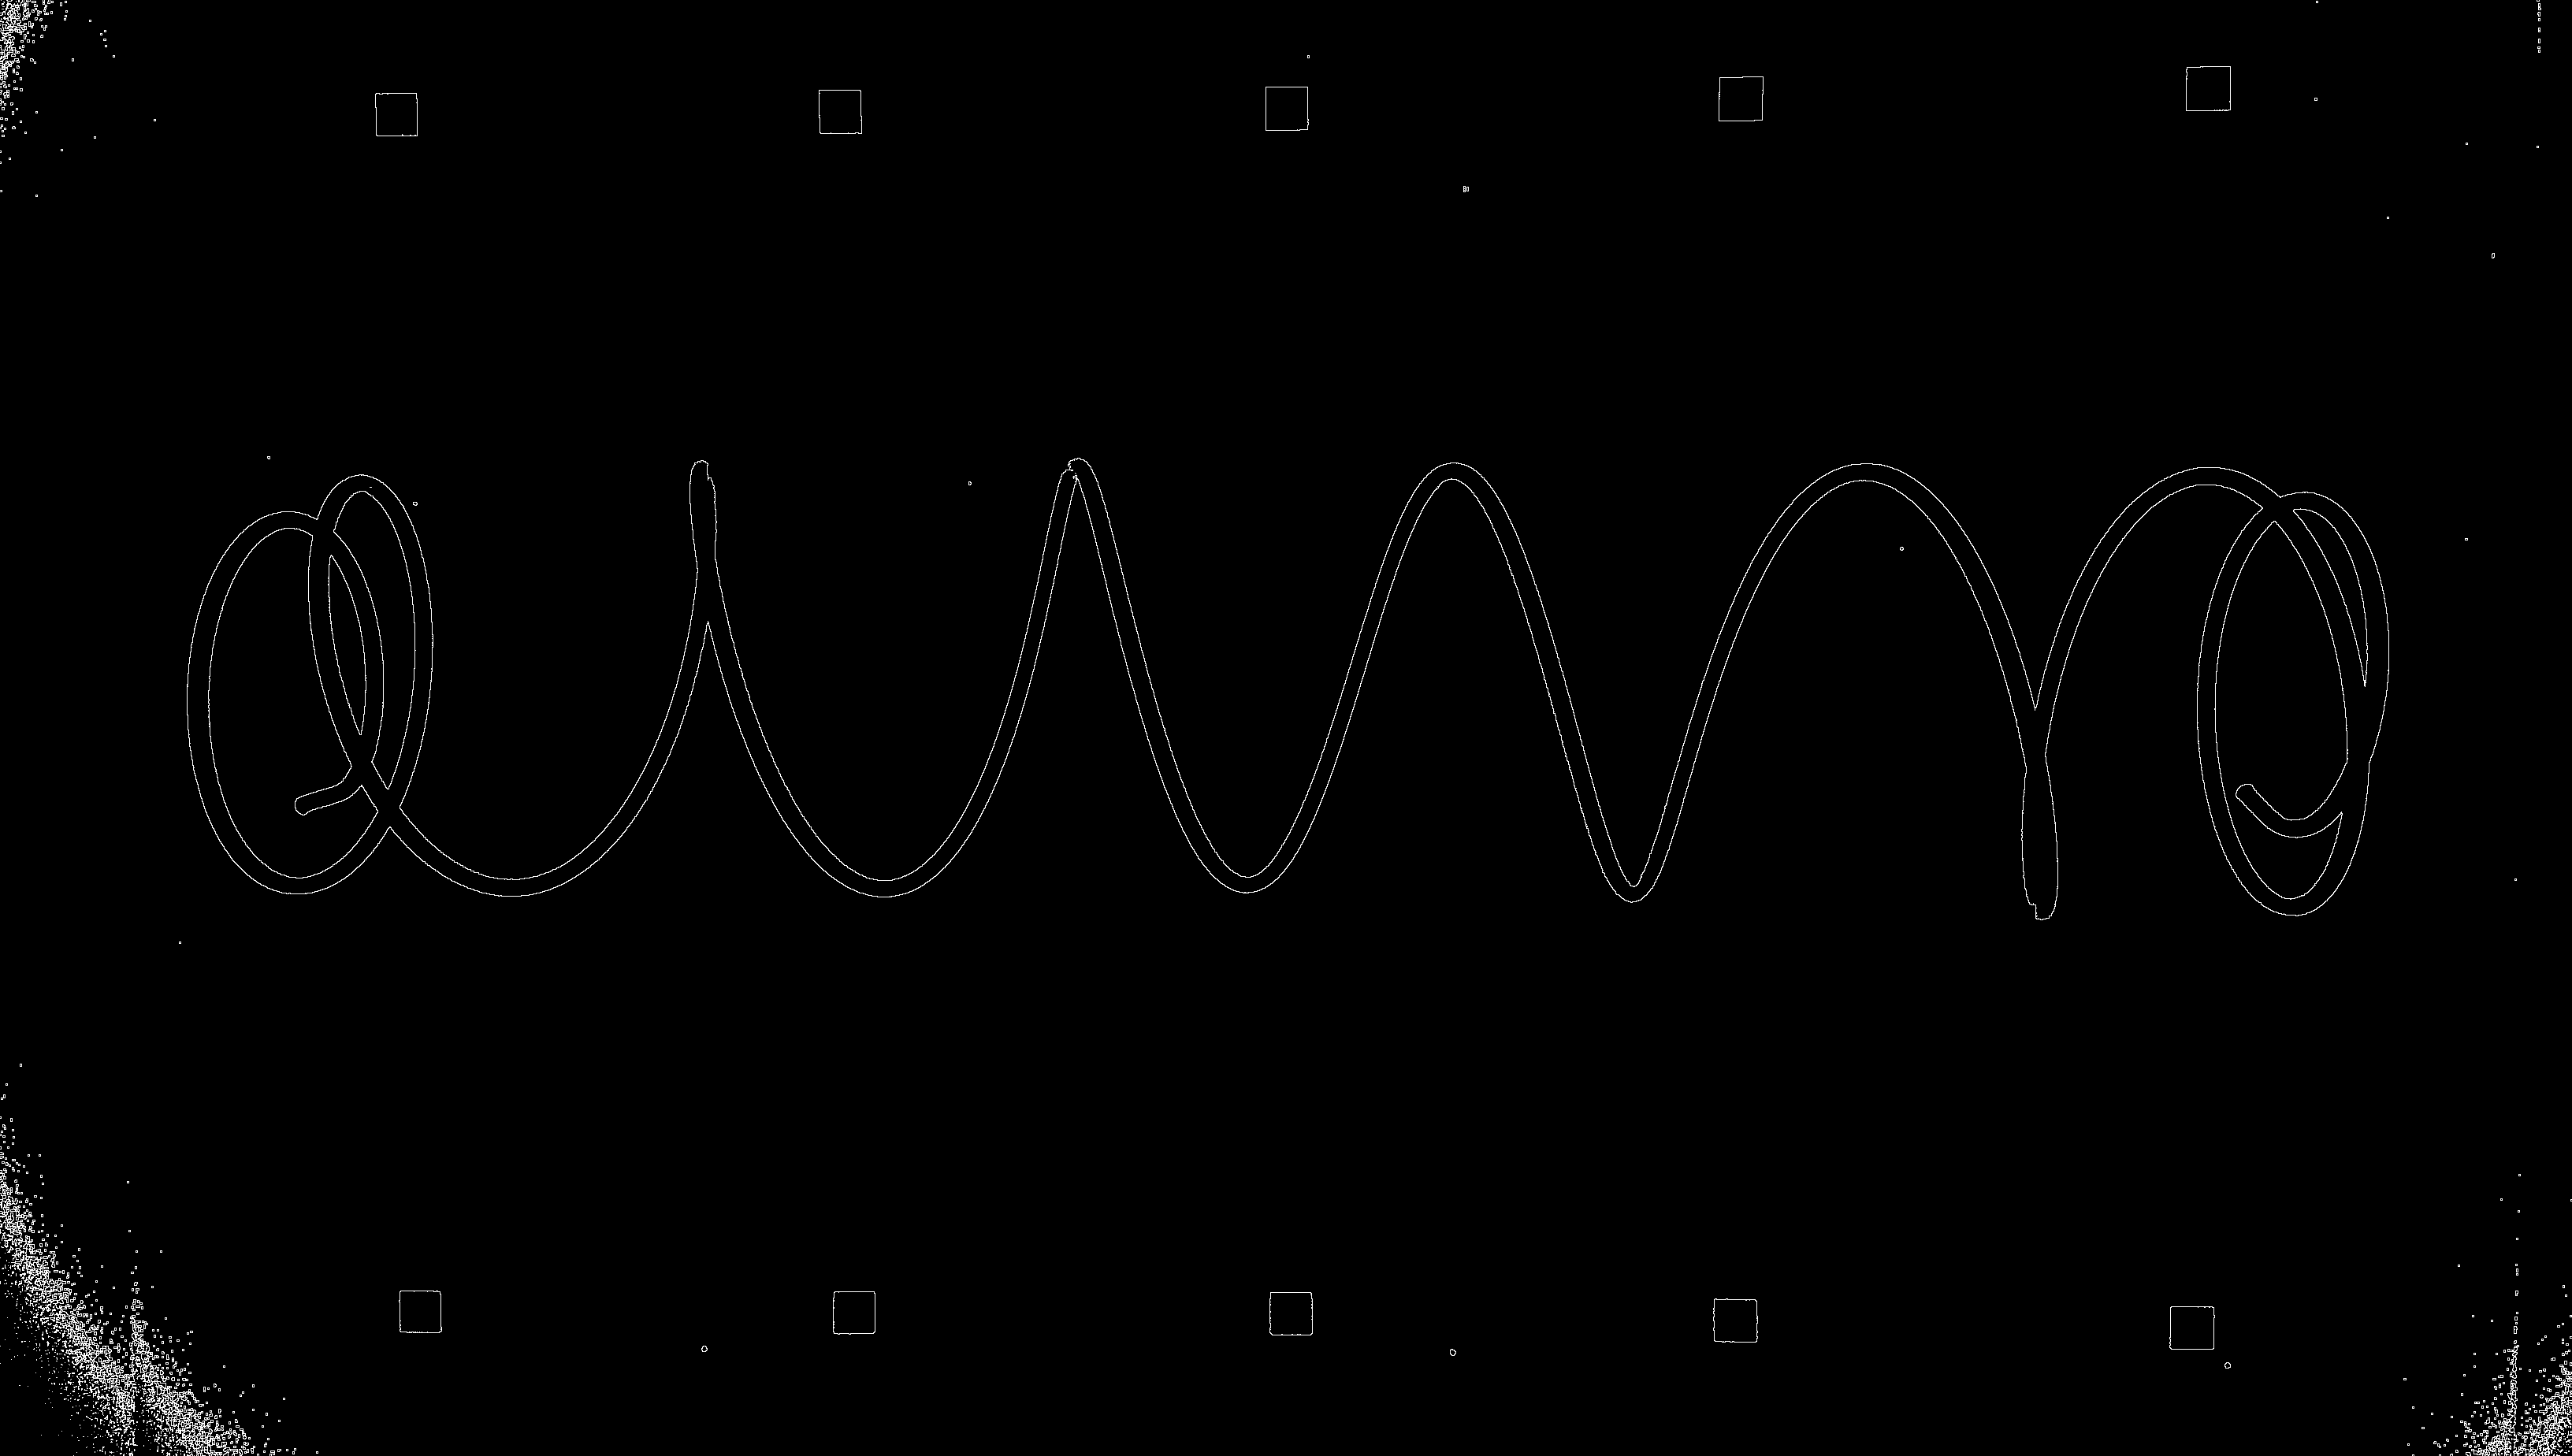
\includegraphics[width=0.9\linewidth]{3-development/threshold/edge.png}}
	\caption{Edges of given image with morphological detection}
	\label{development:edge}
\end{figure}
As we see the image \ref{development:edge} if a noise is bigger than the 3x3 kernel we also receiving the edge of this particular noise. But since we know that our spring cant be located outside of our detection pattern we know we just have to ignore the edges of the image and the small noise in the following steps of calculation.  
\newpage